\section{NEMO Setup}

\subsection{Installation}


Step to install NEMO:
Note: Wavemaker has been used and tested on windows 7. There is a version available for Mac. To use wavemaker, basic web development skills are required (e.g. html, css, javascript).
\begin{itemize}
\item Need first to install and start MARS services v2.0, please see MARS manual. NEMO is currently using three services Network Query Service (NQS), Network Search Service (NSS) and Network Workflow Service (NWS). 
\item NEMO v1 is developed using Wavemaker framework. Need to checkout/download the NEMO (.war and .zip files) from git repo. Git URL is https://ndsslgit.vbi.vt.edu/software-knowledge-discovery/kd-01.git
\item Start Wavemaker on local machine using desktop launcher tool. See Figure~\ref{fig:launcher}. Note: the server will start automatically. Once started, the default browser will open automatically with the wavemaker landing page.

\begin{figure}[H]
\centering
%\label{fig:ebola-kshell-not-effective}
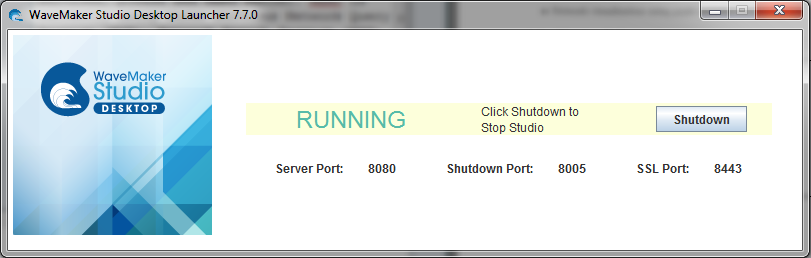
\includegraphics[trim = 0.0in 0.0in 0.0in 0.0in,scale=0.4]{launcher}
\caption{
Wavemaker desktop launcher
}   %   
\label{fig:launcher}
\end{figure}

\item Once Wavemaker framework started, use the import feature to load the .zip file into your working environment, and name the project NEMO.

\begin{figure}[H]
\centering
%\label{fig:ebola-kshell-not-effective}
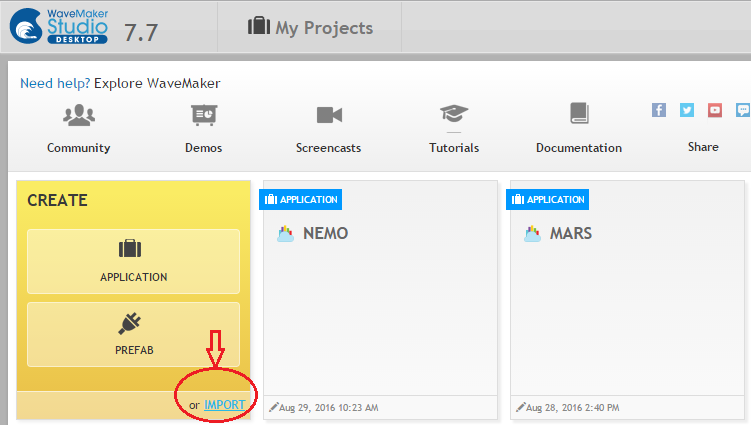
\includegraphics[trim = 0.0in 0.0in 0.0in 0.0in,scale=0.6]{import}
\caption{
Import project in Wavemaker.
}   %   
\label{fig:import}
\end{figure}

\end{itemize}

Steps to setup Netviewer:
Note: NEMO is using a network visualization web application (netviewer). Netviewer is a thin-layer using Gephi and GEXF viewer. 
\begin{itemize}
\item Convert the network .uel file to .csv format.
\item Import the .csv file to gephi. Note: gephi has to be installed on your local machine.
\item Use any visualization or layout algorithm of choice to generate a visualization of the network. Please see gephi manual for different functionality.
\item Once done, click $file->export->graph$ file and choose .gexf. Name the file exactly as the network name.
\item Place the .gexf file under the netviewer dirctory.


\end{itemize}
The app is currently deployed on edisondev VM at /apps/apache-tomcat-7.0.40/webapps/netviewer. The code for the app is available in the git repo at src/netviewer. To deploy netviewer just upload the folder netviewer to the required webapp dir on the VM. 